\documentclass[a4paper]{article}
\usepackage[utf8]{inputenc}
\usepackage{ngerman}
\usepackage{anfpralayout}
\usepackage{physictools}
\usepackage{texcalc}
\usepackage{graphicx}
\usepackage{amsmath}
\usepackage{hyperref}

\setlength{\parindent}{0cm}

\newcommand{\texcalc}{{\TeX}calc}
\begin{document}
\title{Anleitung zu den {\TeX}calc \LaTeXe-Packeten}
\author{Hans Freitag (und einige andere)}
\maketitle

Dieses Dokument gibts als PDF zum Downloaden auf \url{http://www.nawi.at/~zem/texcalc/texcalc.de.pdf}

\image{texcalc.png}{Ein Screenshot des texcalc.py Taschenrechners}

\texcalc Besteht aus drei Komponenten.

\begin{enumerate}
\item texcalc.py ist ein in python geschriebener Taschenrechner der das Pythonmodul
		uncertainties benutzt.
\item texcalc.sty ist ein \LaTeXe-Packet mit dem Berechnungen mit Messunsicherheiten
		direkt aus dem \LaTeXe Dokument heraus möglich sind.
\item Zusatz styles die zwar nicht direkt etwas mit \texcalc zu tun haben, aber für
		das Schreiben von Physikprotokollen Nützlich sein können. Die beiden zusatzpackete
		gliedern sich in:
	\begin{itemize}
	\item physictools.sty eine allgemeine toolsammlung die das Leben leichter machen soll
	\item anfpralayout.sty Layoutparameter Deckbletter etc, die wahrscheinlich nie einmal
		irgendwo anders als an der Uniwien in der Physik verwendet werden.
	\end{itemize}
	Die Contrib Packete sind eine Sammlung von \LaTeXe-Makros von Studierenden der Fakultät,
	die sich im Laufe des Studiums als Hilfreich erwiesen haben.
\end{enumerate}

\tableofcontents

\section{Features/Benutzung}

\subsection{Taschenrechner}

Der Taschenrechner wird mit dem Komando texcalc.py gestartet\footnote{Doppelklick geht auf Windows auch}.

Abbildung \ref{texcalc.png} zeigt einen Screenshot des Taschenrechners an. Zahlen mit Unsicherheiten können
durch $f(number, uncertainty)$ notiert werden. In dem Prompt kann alles berechnet werden was in Python berechnet
werden kann. \\

\subsection{Berechnungen direkt im \LaTeX File}

Die Rechnungen können auch direkt im LaTeX File durchgeführt werden, indem sie innerhalb des calc environments
notiert werden\footnote{\textbackslash usepackage\{texcalc\} nicht vergessen.}

\begin{verbatim}
	\begin{calc}
	x=f(23.55,0.02)
	#r 23.55+/-0.02
	def foo(x):
		y=x**2
		return y

	z=33
	#r 33
	foo(z)
	#r 1089
	y=f(222.0,22)
	#r 222.0+/-22.0

	a=f(24423.0,220)
	#r 222.0+/-22.0
	\end{calc}
\end{verbatim}

\begin{calc}
x=f(23.55,0.02)
#r 23.55+/-0.02
def foo(x):
	y=x**2
	return y

z=33
#r 33
foo(z)
#r 1089
y=f(222.0,22)
#r 222.0+/-22.0

a=f(24423.0,220)
#r 24423.0+/-220.0
\end{calc}

Die \#r kommentarzeilen werden von texcalc.py automatisch eingefügt um die Fehlersuche und die Übersicht zu erleichtern.
Sie enthalten das Ergebnis der letzten Variablenzuweisung bzw des letzten Statements. \\

Die errechneten Werte können jetzt mit dem val komando im Dokument verwendet werden. Der Parameter $[2]$ gibt dabei bei
einer normalen Zahl die zu rundenden Nachkommastellen an. Bei einer Zahl mit Unsicherheit gibt er die Anzahl der
Signifikanten Stellen an, die dann automatisch gerundet und eingefügt werden. Default ist 2. Beispiel: \\

\begin{verbatim}
	$$x_{5sigDigits}=\val[5]{x}$$
	$$x_{2sigDigits}=\val{x}$$
	$$x^2=\val{foo(x)}$$
	$$z=\val{z}$$
	$$y=\val{y}$$
	$$a=\val{a}$$
\end{verbatim}

Wird zu:

$$x_{5sigDigits}=\val[5]{x}$$
$$x_{2sigDigits}=\val{x}$$
$$x^2=\val{foo(x)}$$
$$z=\val{z}$$
$$y=\val{y}$$
$$a=\val{a}$$

Übersetzt werden kann ein solches \LaTeX File mit folgenden Komandos: \\

\begin{verbatim}
	texcalc.py Datei.tex                 --> Fügt die #r kommentarzeilen ein
	texcalc.py -c Datei.tex              --> erzeugt ein pdf texcalc ruft pdflatex auf
	pdflatex --shell-escape Datei.tex    --> Erzeigt ein pdf pdflatex ruft texcalc auf
	lualatex --shell-escape Datei.tex    --> Das gleiche wie pdflatex
	texcalc.py -C -y Datei.tex           --> Wie -c nur werden alle \val{} fest durch die
	                                         werte ersetzt, der prozess ist nicht reversibel,
	                                         aber nützlich um schnell noch manuelle aenderungen
	                                         vorzunehmen.
\end{verbatim}

\section{Download}

\subsection{Abhängigkeiten}

\begin{itemize}
\item Eine LaTeX Distribution wie MikTeX oder TeXlive
\item Python
\item Python-numpy
\item Python-uncertainties
\end{itemize}

\subsection{Dieses Packet}

\begin{itemize}
	\item Download der aktuellen Version von GitHUB \url{https://github.com/zem/texcalc/archive/master.zip}
\end{itemize}

\subsection{Software für Windows}

\subsubsection{\LaTeX}

Da \texcalc auf \LaTeX aufsetzt, ist eine \LaTeX Umgebung erforderlich, außer du beschränkst
dich auf die Funktion als Taschenrechner. MikTex ist eine gute wahl, dazu optional Texnicenter
als Arbeitsumgebung, in der Version 2.0 Beta.

\begin{itemize}
\item \url{http://mirrors.ctan.org/systems/win32/miktex/setup/basic-miktex-2.9.4813.exe}
\item \url{http://sourceforge.net/projects/texniccenter/files/TeXnicCenter/2%20Beta%201/TXCSetup_2Beta1_Win32.exe/download}
\end{itemize}

An dieser Stelle wird auch empfohlen ein Versionskontrollsystem wie GIT zu installieren.

%\subsubsection{Putty und GIT}
%Putty und Puttykeygen
%Brauchst du auch für Fortran übungen. Das ist ein ssh client
%für Windows. GIT braucht den für die Datenübertragung.
%- http://the.earth.li/~sgtatham/putty/latest/x86/putty-0.62-installer.exe
%
%
%git für Windows
%- http://msysgit.googlecode.com/files/Git-1.8.1.2-preview20130201.exe
%	ohne Additional Icons
%	ohne IE integration
%  dann einen dialog später: use tortoise Plink
%
%tortoise git
%Auch hier wieder ein Frontend um die Arbeit leichter zu machen
%- http://tortoisegit.googlecode.com/files/TortoiseGit-1.8.1.0-32bit.msi

\subsection{Python3}

Da TexCalc auf python basiert, brauchst du auch Python, sowie die Module
Numpy und Uncertainties.

\begin{itemize}
\item \url{http://www.python.org/ftp/python/3.3.0/python-3.3.0.msi}
\item \url{http://sourceforge.net/projects/numpy/files/NumPy/1.7.0/numpy-1.7.0-win32-superpack-python3.3.exe/download}
\item \url{http://pypi.python.org/packages/source/u/uncertainties/uncertainties-1.9.tar.gz}
\end{itemize}

Uncertainties kommt als tar archiv ohne grafischen installer daher, damit du das installiert bekommst entpackst du es
ersteinmal in ein verzeichnis, dann führst du cmd.exe aus, und wechselst in das eben angelegte
Verzeichnis\footnote{cd ist das Komando dafür}. Dann führst du "setup.py install" aus.

\subsubsection{\texcalc}

\begin{itemize}
\item \url{https://github.com/zem/texcalc/archive/master.zip}
\end{itemize}

Die Dateien
\begin{itemize}
\item contrib/anfpralayout.sty
\item contrib/physictools.sty
\item texcalc.sty
\end{itemize}
kopierst du nach: \url{C:\backslash Program Files\backslash MiKTeX 2.9\backslash tex\backslash latex\backslash texcalc\backslash}. Den Ordner musst du anlegen.
Die Datei texcalc.py kopierst du nach \url{C:\backslash Program Files\backslash MiKTeX 2.9\backslash miktex\backslash bin\backslash }. \\

Damit die .sty Dateien vom miktex auch gefunden werden, musst du Miktex Optionen als Administrator
ausführen und Rebuild FNTDB machen.\\

Im Texnicenter kannst du unter {\textit ausgabe/ausgabeprofile definieren} das Profil {\textit LatexPDF} kopieren nach {\textit Latex PDF TeXcalc}
als pfad des LaTeX compilers verwendest du:

\begin{verbatim}
	C:\Python33\python.exe "C:\Program Files (x86)\MiKTeX 2.9\miktex\bin\texcalc.py" -c
\end{verbatim}

Zum Schluss legst du noch eine Verknüpfung von \url{C:\backslash Program Files\backslash MiKTeX 2.9\backslash miktex\backslash bin\backslash texcalc.py}
auf den Desktop oder wo du es sonst hinhaben willst.


\subsection{Software für Linux(Debian)}

\begin{verbatim}
	apt-get install texlive latexila python python-numpy python-uncertainties
\end{verbatim}

(Wer will kann und soll natürlich auch vim verwenden, oder meinetwegen auch Emacs.)

\subsection{Entwicklung und Fehlerbehebung}

Mitentwickeln kann jeder. Dafür brauchst du das Versionskontrollsystem GIT
\footnote{GIT ist übrigens auch Prima dafür geeignet um LaTeX dokumente zu verwalten,
sowohl für einen Persönlich als auch wenn mehrere Personen ein Dokument bearbeiten. }
einfach das Repository klonen, entweder von nawi.at:

\begin{verbatim}
	git clone http://www.nawi.at/git/texcalc
\end{verbatim}

Oder über github.com Was sich so tut kannst du im gitweb nachlesen:
\url{http://www.nawi.at/gitweb/?p=texcalc;a=summary} oder halt auf github.com\\

Wenn du einen Patch machen willst kannst du

\begin{verbatim}
	git format-patch origin/master
\end{verbatim}

verwenden, und den Patch an zem@nawi.at mailen oder auf github einen fork
anlegen und patchen.


\section{Installation}

\subsection{Linux}

Installation auf Linux geht mit:

\begin{verbatim}
	make install install-contrib
\end{verbatim}

\subsection{Windows}

Hoffentlich gibts bald ein install.bat script oder sowas. \\

Grundsätzlich müssen alle .sty in miktex eingebunden werden, wie das
geht ist in der MikTex Doku beschrieben:\\

\url{http://docs.miktex.org/manual/localadditions.html}\\
\url{http://docs.miktex.org/manual/texfeatures.html#includedirectory}\\

%\begin{enumerate}
%	\item Erstellen eines Ordners mit dem Namen der \textbf{\textbf{*.sty}}
%		Datei (hier phunivie) unter dem Installationsordner:\\
%
%		\textbf{\emph{MiKTeX\textbackslash tex\textbackslash latex}}\\
%		Normalerweise unter: \textbf{\emph{C:\textbackslash Program
%		Files (x86)\textbackslash MiKTeX 2.9\textbackslash
%		tex\textbackslash latex}}
%	\item Einbinden in Miktex:\\
%			Gehe auf $\boldsymbol{Start \rightarrow MiKTeX \rightarrow
%			Maintenance \rightarrow Settings \rightarrow Refresh~FNDB}$
%
%	\item Fertig!
%\end{enumerate}

Dann muss texcalc.py noch irgendwo hingelegt werden wo es im Pfad liegt, bzw
der Pfad muss angepasst werden. miktex/bin kann funktionieren. ;-)\\


\subsection{Bekannte \texcalc Probleme und deren Lösungen}

\subsubsection{Interger vs float}
\label{integer}

Da \texcalc in python rechnet muss auch den dortigen Datentypen rechnung getragen werden.
Eine Zahl die ohne Kommastelle angegeben wird, wird als Integer (ganze Zahl) interpretiert,
und auch so dividiert. Beispiel:\\

\begin{verbatim}
	>>> 23/4
	5
	>>> 23.0/4.0
	5.75
	>>>
\end{verbatim}

Also am besten immer zahl.0 schreiben.

\section{Contrib}

\subsection{physictools Packet}

In der Preambel:

\begin{verbatim}
	\usepackage{physictools}
\end{verbatim}

\subsubsection{Ergebnis Einleitung}

In der Ergebnisse Section kommen einige sätze immer wieder vor. Hier die Templates:

\begin{verbatim}
	\skalaerr
	\mverr
	\fiterr\usedqti
	\usedgnuplot
	\stopwatcherr
	\multimetererr
	\earthGerr
	\syserr\usedtexcalc
	\\
\end{verbatim}


Und das wird zu: \\

\skalaerr
\mverr
\fiterr\usedqti
\usedgnuplot
\stopwatcherr
\multimetererr
\earthGerr
\syserr\usedtexcalc
\\

Das geht natürlich auch auf Englisch ohne ngerman packet: \\

\selectlanguage{USenglish}

\skalaerr
\mverr
\fiterr\usedqti
\usedgnuplot
\stopwatcherr
\multimetererr
\earthGerr
\syserr\usedtexcalc
\\

\selectlanguage{ngerman}

\subsubsection{image commands}

\begin{verbatim}
	\image{texcalc.png}{Ein Screenshot des texcalc.py Taschenrechners}
\end{verbatim}

is actually a shortcut for:

\begin{verbatim}
	\begin{figure}[h]
	\centering
	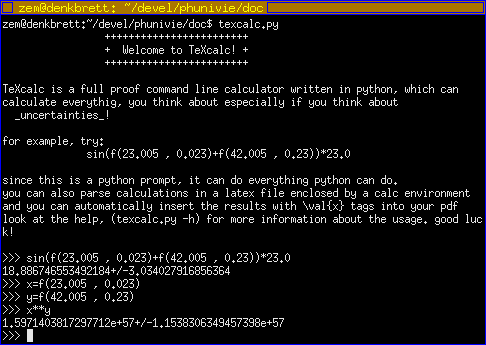
\includegraphics[width=0.7\textwidth]{texcalc.png}
	\caption{Ein Screenshot des texcalc.py Taschenrechners}
	\label{texcalc.png}
	\end{figure}
\end{verbatim}


\subsubsection{$23\E{10}$}

\begin{verbatim}
$$23\E{10}$$
\end{verbatim}

\subsubsection{\ddt}

\begin{verbatim}
$$
	\ddt
$$
\end{verbatim}

\subsubsection{$\dnach{x}$}

\begin{verbatim}
$$
	\dnach{x}
$$
\end{verbatim}

\subsubsection{$\ddnach{x}{y}$}

\begin{verbatim}
$$
	\ddnach{x}{y}
$$
\end{verbatim}


\subsubsection{$\dddnach{x}{y}{z}$}

\begin{verbatim}
$$
	\dddnach{x}{y}{z}
$$
\end{verbatim}

\subsubsection{$\dznach{x}{y}$}

\begin{verbatim}
$$
	\dznach{x}{y}
$$
\end{verbatim}

\subsubsection{$\vnabla$}

\begin{verbatim}
$$
	\vnabla
$$
\end{verbatim}

\subsubsection{$\evec{x}$}

\begin{verbatim}
$$
	\evec{x}
$$
\end{verbatim}

\subsubsection{$\bra{x}$}

\begin{verbatim}
$$
	\bra{x}
$$
\end{verbatim}

\subsubsection{$\ket{x}$}

\begin{verbatim}
$$
	\ket{x}
$$
\end{verbatim}

\subsubsection{$\bracket{x}{y}$}

\begin{verbatim}
$$
	\bracket{x}{y}
$$
\end{verbatim}

\subsubsection{$\up$}

\begin{verbatim}
$$
	\up
$$
\end{verbatim}

\subsubsection{$\down$}

\begin{verbatim}
$$
	\down
$$
\end{verbatim}

\subsubsection{$\upup$}

\begin{verbatim}
$$
	\upup
$$
\end{verbatim}

\subsubsection{$\downdown$}

\begin{verbatim}
$$
	\downdown
$$
\end{verbatim}

\subsubsection{$\sandwich{x}{y}$}

\begin{verbatim}
$$
	\sandwich{x}{y}
$$
\end{verbatim}

\subsubsection{$\fsqrt{x}{y}$}

\begin{verbatim}
$$
	\fsqrt{x}{y}
$$
\end{verbatim}



%%%%%%%%%%%%%%%%%%%%%%%%%%%%%%%%%%%%%%%%%%%%%%%%%%%%%%%%%%%%%%%%%%%%%%%%%%%%%%%%%%%%%%%%%%%%%%%%%%%%%%%%%%%%%%%%
\subsection{anfpralayout}
%%%%%%%%%%%%%%%%%%%%%%%%%%%%%%%%%%%%%%%%%%%%%%%%%%%%%%%%%%%%%%%%%%%%%%%%%%%%%%%%%%%%%%%%%%%%%%%%%%%%%%%%%%%%%%%%

In der Preambel:

\begin{verbatim}
	\usepackage{anfpralayout}
\end{verbatim}

oder

\begin{verbatim}
	\usepackage[option]{anfpralayout}
\end{verbatim}

Optionen können sein:

\begin{description}
	\item[basti] Sebastians Layout Parameter (margin$=$2.5cm)
	\item[motz] Motz's Layout Parameter
\end{description}


\subsubsection{Titelseite}

Für das Anfängerpraktikum ist eine Besondere Titelseite nötig, die
kann natürlich ganz einfach gesetzt werden:

\begin{verbatim}
\semester{SoSe 2011}
%\fakulty{Fakultät für Sonstwas}
%\title{Physikalisches Praktikum\\für Lehramtskandidaten}
\experiment{1. Fnord}
%\date{abgabedatum}
\author{Hans Freitag}
\group{3}
\supervisor{someone}

\makeanfpratitle
\end{verbatim}

Die auskommentierten Parameter sind optional. Und so siehts
aus\footnote{$\backslash$date und $\backslash$author gehen zur Zeit nur wenn der Block am
Anfang eines Dokumentes steht}:

\semester{SoSe 2011}
%\fakulty{Fakultät für Sonstwas}
%\title{Physikalisches Praktikum\\für Lehramtskandidaten}
\experiment{1. Fnord}
%\date{\today}
%\author{Hans Freitag}
\group{3}
\supervisor{someone}
\makeanfpratitle


\end{document}
